\documentclass{beamer}
\mode<presentation>
\usepackage{amsmath,amssymb,mathtools}
\usepackage{textcomp}
\usepackage{gensymb}
\usepackage{adjustbox}
\usepackage{subcaption}
\usepackage{enumitem}
\usepackage{multicol}
\usepackage{listings}
\usepackage{url}
\usepackage{graphicx} % <-- needed for images
\def\UrlBreaks{\do\/\do-}

\usetheme{Boadilla}
\usecolortheme{lily}
\setbeamertemplate{footline}{
  \leavevmode%
  \hbox{%
  \begin{beamercolorbox}[wd=\paperwidth,ht=2ex,dp=1ex,right]{author in head/foot}%
    \insertframenumber{} / \inserttotalframenumber\hspace*{2ex}
  \end{beamercolorbox}}%
  \vskip0pt%
}
\setbeamertemplate{navigation symbols}{}

\lstset{
  frame=single,
  breaklines=true,
  columns=fullflexible,
  basicstyle=\ttfamily\tiny   % tiny font so code fits
}

\numberwithin{equation}{section}

% ---- your macros ----
\providecommand{\nCr}[2]{\,^{#1}C_{#2}}
\providecommand{\nPr}[2]{\,^{#1}P_{#2}}
\providecommand{\mbf}{\mathbf}
\providecommand{\pr}[1]{\ensuremath{\Pr\left(#1\right)}}
\providecommand{\qfunc}[1]{\ensuremath{Q\left(#1\right)}}
\providecommand{\sbrak}[1]{\ensuremath{{}\left[#1\right]}}
\providecommand{\lsbrak}[1]{\ensuremath{{}\left[#1\right.}}
\providecommand{\rsbrak}[1]{\ensuremath{\left.#1\right]}}
\providecommand{\brak}[1]{\ensuremath{\left(#1\right)}}
\providecommand{\lbrak}[1]{\ensuremath{\left(#1\right.}}
\providecommand{\rbrak}[1]{\ensuremath{\left.#1\right)}}
\providecommand{\cbrak}[1]{\ensuremath{\left\{#1\right\}}}
\providecommand{\lcbrak}[1]{\ensuremath{\left\{#1\right.}}
\providecommand{\rcbrak}[1]{\ensuremath{\left.#1\right\}}}
\theoremstyle{remark}
\newtheorem{rem}{Remark}
\newcommand{\sgn}{\mathop{\mathrm{sgn}}}
\providecommand{\abs}[1]{\left\vert#1\right\vert}
\providecommand{\res}[1]{\Res\displaylimits_{#1}}
\providecommand{\norm}[1]{\lVert#1\rVert}
\providecommand{\mtx}[1]{\mathbf{#1}}
\providecommand{\mean}[1]{E\left[ #1 \right]}
\providecommand{\fourier}{\overset{\mathcal{F}}{ \rightleftharpoons}}
\providecommand{\system}{\overset{\mathcal{H}}{ \longleftrightarrow}}
\providecommand{\dec}[2]{\ensuremath{\overset{#1}{\underset{#2}{\gtrless}}}}
\newcommand{\myvec}[1]{\ensuremath{\begin{pmatrix}#1\end{pmatrix}}}
\let\vec\mathbf

\title{Matgeo Presentation - Problem 2.5.31}
\author{ee25btech11063 - Vejith}

\begin{document}


\frame{\titlepage}
\begin{frame}{Question}
If two vertices of an equilateral triangle are \brak{3,0} and \brak{6,0},find the third vertex
\end{frame}

\begin{frame}{Description}
\textbf{Solution: }\\
\begin{table}[h!]    
  \centering
  \begin{table}[htbp]
  \centering
  \caption{Table-3}
  \label{table3}
  \begin{tabular}{cc}
  \textbf{Processing Technique} & \textbf{Producct} \\ \\
    P. Calendering & 1. Pipes \\
    Q. Extrusion & 2. Disposable cups \\
    R. Injection moulding & 3. Sheets \\
    S. Thermoforming & 4. Nylon gears \\
  \end{tabular}
\end{table}
  \caption{Variables Used}
  \label{}
\end{table}
\end{frame}

\begin{frame}{Solution}
\begin{align}
   \text{ The vector joining from }\Vec{A}\ \text{to } \Vec{B} \text{ is given by } \Vec{B}-\Vec{A}=\myvec{6\\0}-\myvec{3\\0}\\
\implies \Vec{B}-\vec{A}=\myvec{3\\0}.\\
\end{align}

An equilateral triangle can be obtained by rotating $\Vec{B}$-$\vec{A}$ by $\Vec{A}$ about $+60\degree$ or $-60\degree$ .The rotation matrix $\vec{P}$ at angle $\theta$ is defined as\\
\vspace{0.5cm}
\begin{align}
    \vec{P}(\theta)=\myvec{
   \cos \theta & -\sin \theta
    \\
   \sin \theta & \cos \theta
   }\\
\end{align}
\end{frame}

\begin{frame}{Solution}
\begin{align}
    \vec{P}(60\degree)=\myvec{
   \frac{1}{2} & \frac{-\sqrt{3}}{2}
    \\
   \frac{\sqrt{3}}{2} & \frac{1}{2}
   } \hspace{3cm}
   \vec{P}(-60\degree)=\myvec{
   \frac{1}{2} & \frac{\sqrt{3}}{2}
    \\
   \frac{-\sqrt{3}}{2} & \frac{1}{2}
   }\\
\end{align}
Apply $\vec{P}$($60\degree$) or $\vec{P}$($-60\degree$) to $\Vec{B}-\vec{A}$ and add it to $\Vec{A}$ to get $\vec{C}$\\
\begin{align}
    \vec{C}=\vec{A}+\vec{P}(60\degree)(\Vec{B}-\vec{A})\hspace{1cm} \text{or} \hspace{1cm}\vec{C}=\vec{A}+\vec{P}(-60\degree)(\Vec{B}-\vec{A})\hspace{2cm}\\
    \vec{P}(60\degree)\myvec{3\\0}=\myvec{\frac{3}{2}\\\frac{3\sqrt{3}}{2}} \hspace{1cm} \text{or} \hspace{2.8cm} \vec{P}(-60\degree)\myvec{3\\0}=\myvec{\frac{3}{2}\\\frac{-3\sqrt{3}}{2}}\\
    \end{align}
\end{frame}
\begin{frame}{Conclusion and Plot}
\begin{align}
    \vec{C}=\myvec{\frac{3}{2}\\\frac{3\sqrt{3}}{2}} \hspace{2.5cm} \text{or} \hspace{4.6cm} \vec{C}=\myvec{\frac{3}{2}\\\frac{-3\sqrt{3}}{2}}
\end{align}
\begin{figure}[H]
    \centering
    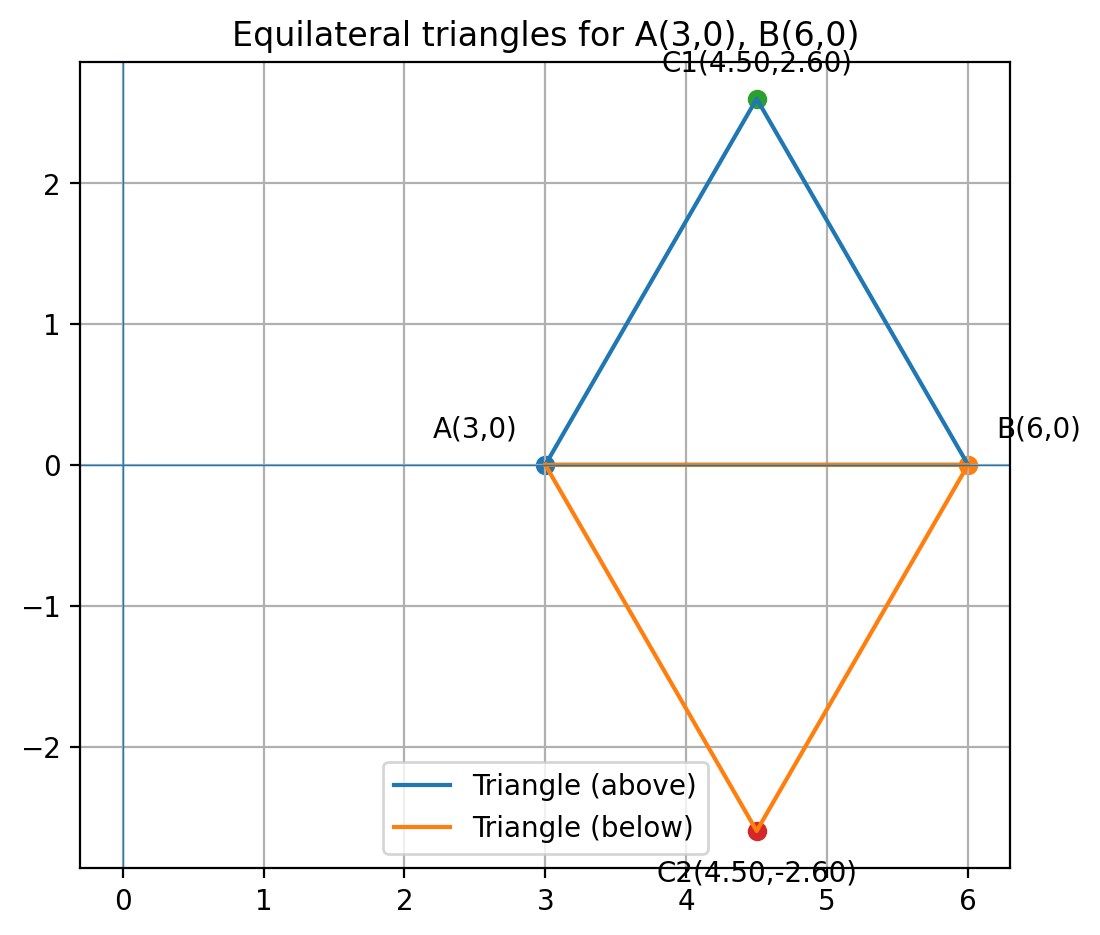
\includegraphics[width=0.5\columnwidth]{figs/01.png}
    \label{fig-1}
\end{figure}
\end{frame}


% --------- CODE APPENDIX ---------
\section*{Appendix: Code}

% C program
\begin{frame}[fragile]{C Code: code.c}
\begin{lstlisting}[language=C]
#include <stdio.h>
#include <math.h>

int main() {
    FILE *fp;
    fp = fopen("triangle.dat", "w");
    if (fp == NULL) {
        printf("Error opening file!\n");
        return 1;
    }

    // Given vertices
    double x1 = 3, y1 = 0;
    double x2 = 6, y2 = 0;

    // Midpoint of AB
    double xm = (x1 + x2) / 2.0;
    double ym = (y1 + y2) / 2.0;

    // Length of AB
    double side = sqrt((x2 - x1)*(x2 - x1) + (y2 - y1)*(y2 - y1));

    // Height of equilateral triangle
    double h = (sqrt(3) / 2.0) * side;

    // Two possible third vertices
    double x3a = xm;
    double y3a = ym + h;

    double x3b = xm;
    double y3b = ym - h;

    // Writing results to file
    \end{lstlisting}
\end{frame}

\begin{frame}[fragile]{C Code: code.c}
\begin{lstlisting}[language=C]
    fprintf(fp, "First vertex: (%.2f, %.2f)\n", x1, y1);
    fprintf(fp, "Second vertex: (%.2f, %.2f)\n", x2, y2);
    fprintf(fp, "Third vertex (above x-axis): (%.2f, %.2f)\n", x3a, y3a);
    fprintf(fp, "Third vertex (below x-axis): (%.2f, %.2f)\n", x3b, y3b);

    fclose(fp);

    printf("Results written to triangle.dat successfully.\n");
    return 0;
}
\end{lstlisting}
\end{frame}


\begin{frame}[fragile]{Python: plot.py}
\begin{lstlisting}[language=Python]
   import numpy as np
import matplotlib.pyplot as plt

# Given vertices
A = np.array([3.0, 0.0])
B = np.array([6.0, 0.0])

# Midpoint and side/height
M = (A + B) / 2
AB = B - A
side = np.linalg.norm(AB)
h = (np.sqrt(3) / 2) * side

# Unit vector perpendicular to AB
perp = np.array([-AB[1], AB[0]]) / np.linalg.norm(AB)

# Two possible third vertices
C1 = M + h * perp   # above x-axis
C2 = M - h * perp   # below x-axis

fig, ax = plt.subplots(figsize=(6, 6))

# Plot triangles (above and below)
ax.plot([A[0], B[0], C1[0], A[0]], [A[1], B[1], C1[1], A[1]], label="Triangle (above)")
ax.plot([A[0], B[0], C2[0], A[0]], [A[1], B[1], C2[1], A[1]], label="Triangle (below)")

# Mark points
for p in (A, B, C1, C2):
    ax.scatter(p[0], p[1])

# Label points (use annotate to offset labels)
ax.annotate("A(3,0)", xy=A, xytext=(-10, 8), textcoords="offset points", ha="right", va="bottom")
ax.annotate("B(6,0)", xy=B, xytext=(10, 8), textcoords="offset points", ha="left", va="bottom")
\end{lstlisting}
\end{frame}

\begin{frame}[fragile]{Python: plot.py}
\begin{lstlisting}[language=Python]
ax.annotate(f"C1({C1[0]:.2f},{C1[1]:.2f})", xy=C1, xytext=(0, 8), textcoords="offset points", ha="center", va="bottom")
ax.annotate(f"C2({C2[0]:.2f},{C2[1]:.2f})", xy=C2, xytext=(0, -10), textcoords="offset points", ha="center", va="top")

# Axes/formatting
ax.axhline(0, linewidth=0.5)
ax.axvline(0, linewidth=0.5)
ax.set_aspect('equal', adjustable='box')
ax.grid(True)
ax.legend()
ax.set_title("Equilateral triangles for A(3,0), B(6,0)")

# Save and show
plt.savefig("triangle.png", dpi=200, bbox_inches="tight")
plt.show()
\end{lstlisting}
\end{frame}
\end{document}
